\documentclass[xcolor=x11names,compress]{beamer}

%\newcommand*{\upbullet}{\includegraphics[width=1em]{QC8_8.3_psi.pdf}}
%\setbeamertemplate{itemize item}{\upbullet}

%% General document %%%%%%%%%%%%%%%%%%%%%%%%%%%%%%%%%%
\usepackage{graphicx}
\usepackage{tikz}
\usetikzlibrary{decorations.fractals}
\usetikzlibrary{arrows,shapes}
\usetikzlibrary{shapes.geometric}
\usetikzlibrary{shadows}
\usetikzlibrary{snakes}
\usetikzlibrary{decorations.text}
\usepackage{fancybox}
\usepackage{amsmath}
\usepackage{graphics}
\usepackage[latin1]{inputenc}
\usefonttheme{professionalfonts}
\usepackage{times}
\usepackage{verbatim}
\usepackage{ragged2e}
\usepackage[justification=centering]{caption}
\usepackage{fancybox}
\usepackage{CJK}
\usepackage{media9}

%% Beamer Layout %%%%%%%%%%%%%%%%%%%%%%%%%%%%%%%%%%

\useoutertheme[subsection=false, shadow]{miniframes}
\useinnertheme{default}
\usefonttheme{serif}
\usepackage{palatino}

\setbeamercovered{transparent}  	%<<<<<----------------- This sets transparent itemized lists.
\usefonttheme[onlymath]{serif}   	%<<<<<----------------- Sets the font only for formulas.

\setbeamerfont{title like}{shape=\scshape}
\setbeamerfont{frametitle}{shape=\scshape}

\setbeamercolor*{lower separation line head}{bg=DeepSkyBlue4} 
\setbeamercolor*{normal text}{fg=black,bg=white} 
\setbeamercolor*{alerted text}{fg=red} 
\setbeamercolor*{example text}{fg=black} 
\setbeamercolor*{structure}{fg=black} 
 
\setbeamercolor*{palette tertiary}{fg=black,bg=black!10} 
\setbeamercolor*{palette quaternary}{fg=black,bg=black!10} 

\renewcommand{\(}{\begin{columns}}
\renewcommand{\)}{\end{columns}}
\newcommand{\<}[1]{\begin{column}{#1}}
\renewcommand{\>}{\end{column}}
\setbeamertemplate{navigation symbols}{}

%\setbeamertemplate{footline}[page number]
\setbeamertemplate{footline}
{
  \leavevmode%
  \hbox{%
  \begin{beamercolorbox}[wd=.28\paperwidth,ht=2.25ex,dp=1ex,center]{author in head/foot}%
    \usebeamerfont{author in head/foot}Joseph M. Fedrow  \end{beamercolorbox}%
  \begin{beamercolorbox}[wd=.44\paperwidth,ht=2.25ex,dp=1ex,center]{title in head/foot}%
    \usebeamerfont{title in head/foot}Git and LaTeX for Your Scientific Workflow \end{beamercolorbox}%
  \begin{beamercolorbox}[wd=.28\paperwidth,ht=2.25ex,dp=1ex,right]{date in head/foot}%
    \usebeamerfont{date in head/foot}\insertshortdate{}\hspace*{2em}
    \insertframenumber{} / \inserttotalframenumber\hspace*{2ex} 
  \end{beamercolorbox}}%
  \vskip0pt%
}


%%%%%%%%%%%%%%%%%%%%%%%%%%%%%%%%%%%%%%%%%%%%%%%%%%%%%%
%
%
\begin{document} 

\section{\scshape Introduction}
\subsection{Introduction}

\begin{frame}
\vspace{-0.5cm}
\title{
Git Your LaTeX On!
}\author{
	Joseph M. Fedrow\\
	\vspace{0.5cm}
	\begin{tikzpicture}[decoration=Koch snowflake]
		\draw[DeepSkyBlue4] decorate{ decorate{ decorate{ (0,0) -- (3,0) }}};
	\end{tikzpicture}
	\vspace{-0.8cm}
}

\date{
	\today
	}
	
	\titlepage
	`
	\vspace{-0.5cm}
	
	
	
	 \centerline{
\includegraphics[scale=0.3]{asu-logo-E9CC4BDF34-seeklogo.com} \hspace{1.115cm}  
\includegraphics[scale=0.18]{asu-logo-DA1C895AD3-seeklogo.com}  \hfill{} 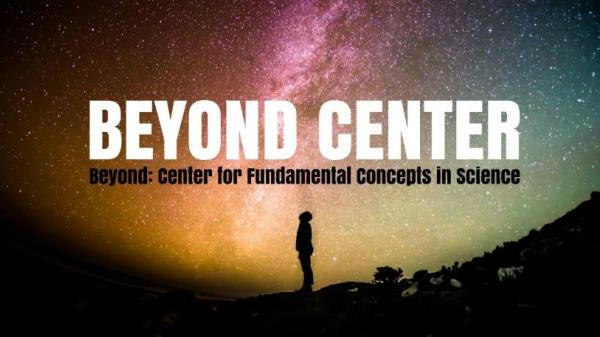
\includegraphics[scale=0.19]{Beyond Center Logo (New)}}

\end{frame}

\frame{
\frametitle{What is Git and LaTeX?}

}

\frame{
\frametitle{How Can They Help You?}

}

\frame{
\frametitle{History of Git}

}

\frame{
\frametitle{History of LaTeX}

}


\section{\scshape Getting Git}
\subsection{Getting Git}


\frame{
\frametitle{How to Use Git}

}

\section{\scshape Typesetting LaTeX}
\subsection{Typesetting LaTeX}

\frame{
\frametitle{How to Use LaTeX}

}
\section{\scshape Summary}
\subsection{Summary}

\frame{
\frametitle{Summary}

}

\end{document}


